\documentclass[12pt, a4paper, oneside]{ctexart}
\usepackage{amsmath, amsthm, amssymb, bm, color, graphicx, geometry, mathrsfs,extarrows, braket, booktabs, array, subfigure}
\usepackage[colorlinks,linkcolor=red,anchorcolor=blue,citecolor=blue,urlcolor=blue,menucolor=black]{hyperref}
\setmainfont{Times New Roman}  % 设置英文字体
\setsansfont{Calibri}
\setmonofont{Consolas}

\linespread{1.4}
%\geometry{left=2.54cm,right=2.54cm,top=3.18cm,bottom=3.18cm}
\geometry{left=1.84cm,right=1.84cm,top=2.18cm,bottom=2.18cm}
\newenvironment{problem}{\par\noindent\textbf{题目. }}{\bigskip\par}
\newenvironment{solution}{\par\noindent\textbf{解答. }}{\bigskip\par}
\newenvironment{note}{\par\noindent\textbf{注记. }}{\bigskip\par}

\everymath{\displaystyle} % 默认全部行间公式
\DeclareMathOperator*\uplim{\overline{lim}} % 定义上极限 \uplim_{}
\DeclareMathOperator*\lowlim{\underline{lim}} % 定义下极限 \lowlim_{}
\let\leq=\leqslant % 将全部leq变为leqslant
\let\geq=\geqslant % geq同理
\graphicspath{{figure/}}

% 一些宏定义
\def\bd{\boldsymbol}    % 加粗(向量) boldsymbol
\def\disp{\displaystyle}% 使用行间公式 displaystyle(默认)
\def\tsty{\textstyle}   % 使用行内公式 textstyle
\def\sign{\text{sign}}  % sign function
\def\wtd{\widetilde}    % 宽波浪线 widetilde
\def\R{\mathbb{R}}      % Real number
\def\C{\mathbb{C}}      % Complex number
\def\d{\mathrm{d}}      % differential operator
\def\e{\mathrm{e}}      % Euler's number
\def\i{\mathrm{i}}      % imaginary number
\def\re{\mathrm{Re\,}}    % Real part
\def\im{\mathrm{Im\,}}    % Imaginary part
\def\L{\mathcal{L}}     % Loss function
\def\wdh{\widehat}      % 宽帽子 widehat
\def\ol{\overline}      % 上横线 overline
\def\ul{\underline}     % 下横线 underline
\def\add{\vspace{1ex}}  % 增加行间距
\def\del{\vspace{-3.5ex}}  % 减少行间距

% 基本信息
\newcommand{\RQ}{\today} % 日期
\newcommand{\km}{经济博弈论} % 科目
\newcommand{\bj}{强基数学002} % 班级
\newcommand{\xm}{吴天阳} % 姓名
\newcommand{\xh}{2204210460} % 学号

\begin{document}

%\pagestyle{empty}
\pagestyle{plain}
\vspace*{-15ex}
\centerline{\begin{tabular}{*5{c}}
    \parbox[t]{0.25\linewidth}{\begin{center}\textbf{日期}\\ \large \textcolor{blue}{\RQ}\end{center}} 
    & \parbox[t]{0.2\linewidth}{\begin{center}\textbf{科目}\\ \large \textcolor{blue}{\km}\end{center}}
    & \parbox[t]{0.2\linewidth}{\begin{center}\textbf{班级}\\ \large \textcolor{blue}{\bj}\end{center}}
    & \parbox[t]{0.1\linewidth}{\begin{center}\textbf{姓名}\\ \large \textcolor{blue}{\xm}\end{center}}
    & \parbox[t]{0.15\linewidth}{\begin{center}\textbf{学号}\\ \large \textcolor{blue}{\xh}\end{center}} \\ \hline
\end{tabular}}
\vspace*{4ex}

% 正文部分
\paragraph{第四章}\del
\paragraph{5.}分析两次重复2.4.2中制式问题(见下图)时双方的均衡策略.
\begin{figure}[htbp]
    \centering
    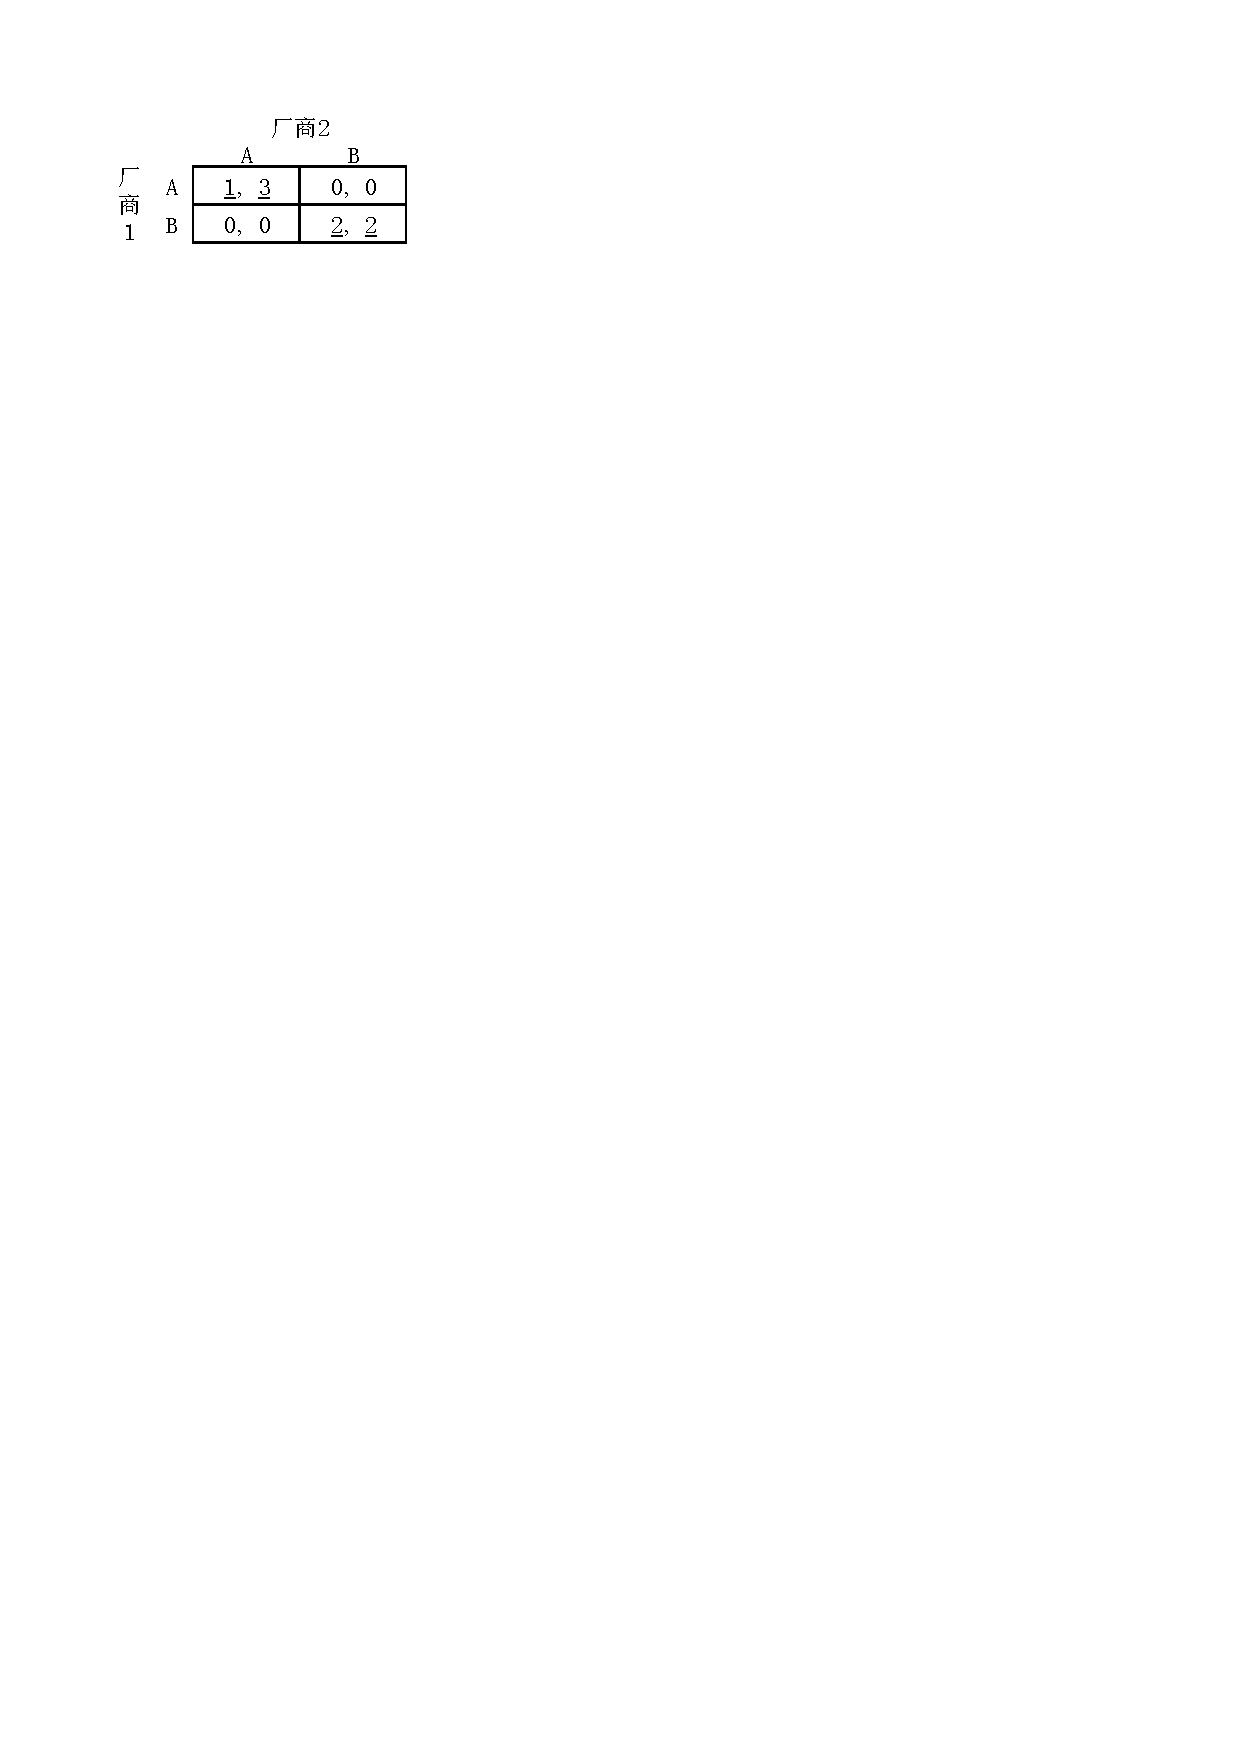
\includegraphics[scale=1]{Economic4.5.pdf}
    \caption{制式问题}
\end{figure}
\begin{solution}
    该博弈有两个纯策略纳什均衡$(A,A)$和$(B,B)$, 而且两个纳什均衡都是Pareto上策均衡, 厂商1偏好$(B,B)$, 厂商1偏好$(A,A)$, 混合纳什均衡的期望得益更低, 决策为$(A,B)$和$(B,A)$.

    根据重复子博弈完美纳什均衡的定义, 上述博弈的完美纳什均衡有很多种, 包括采用纯纳什均衡$(A,A)$或$(B,B)$, 还有重复混合策略纳什均衡. 由于上述博弈没有对双方都有利的策略, 所以重复博弈的结果不完全确定.
\end{solution}

\paragraph{6.}两次重复下面的得益矩阵表示的静态博弈. 如果你是博弈方1, 你会采用怎样的策略?
\begin{figure}[htbp]
    \centering
    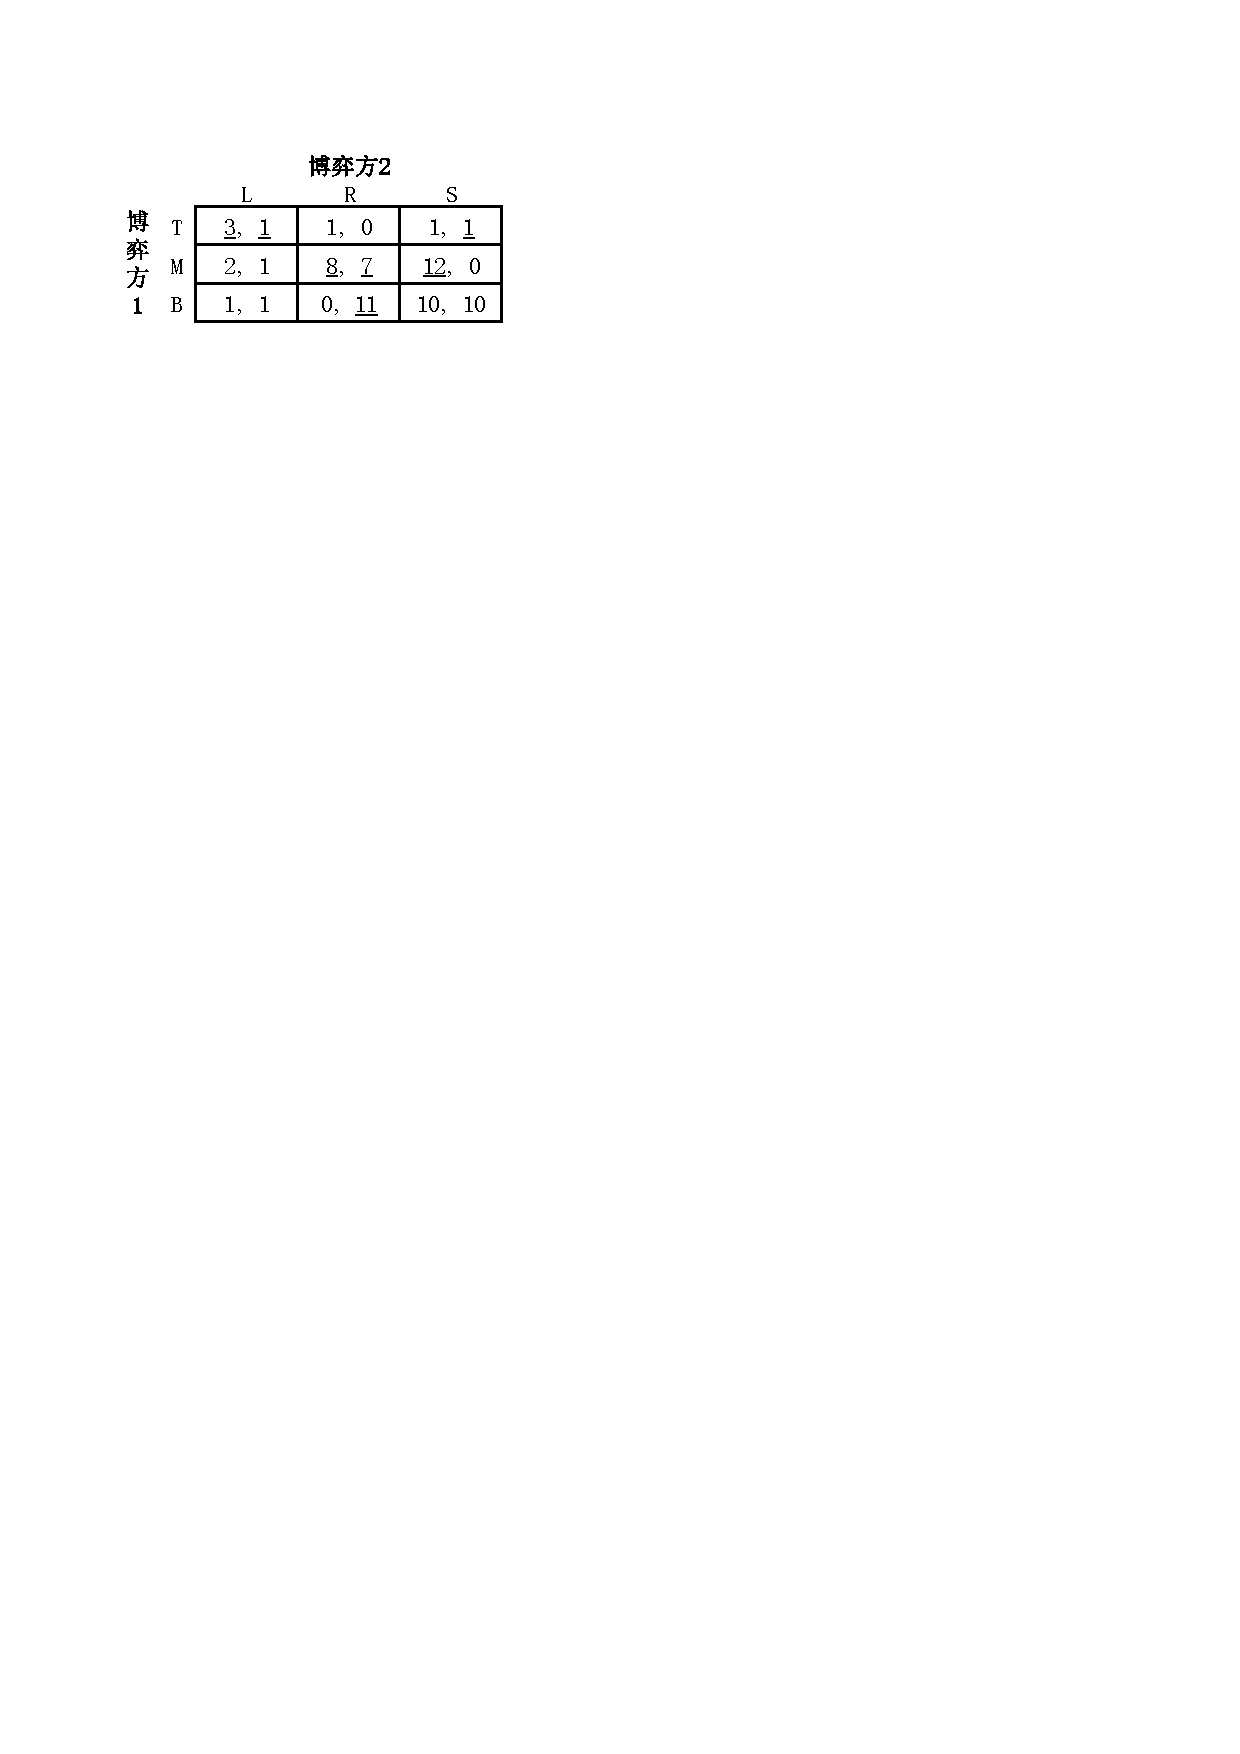
\includegraphics[scale=1]{Economic4.6.pdf}
    \caption{第6题}
\end{figure}
\begin{solution}
    利用划线法可以得到$(T, L)$和$(M,R)$为纯策略纳什均衡, 但这两个策略的得益均小于Pareto上策均衡$(B,S)$. 在重复博弈中, 我们需要努力实现$(B,S)$均衡从而提高自己的利益.

    若我是博弈方1, 第一次选择$B$, 如果结果为$(B,S)$, 则第二次选择$M$, 否则, 根据报复机制, 第二次选择$T$.

    如果博弈方2也具有足够的理性, 则决策结果大概率会为$(B,S)$和$(M,R)$, 使得双方利益最大化.
\end{solution}
\paragraph{7.}两次重复下面这个得益矩阵表示的两人静态博弈. 问能否有一个子博弈完美纳什均衡策略组合, 实现第一阶段的得益是$(4,4)$? 如能, 给出双方的侧率, 如不能, 证明为什么不能. 如果策略组合(下, 左)的得益改为$(1,5)$会发生什么变化? 至少能在部分阶段实现得益$(4,4)$的条件是什么?
\begin{figure}[htbp]
    \centering
    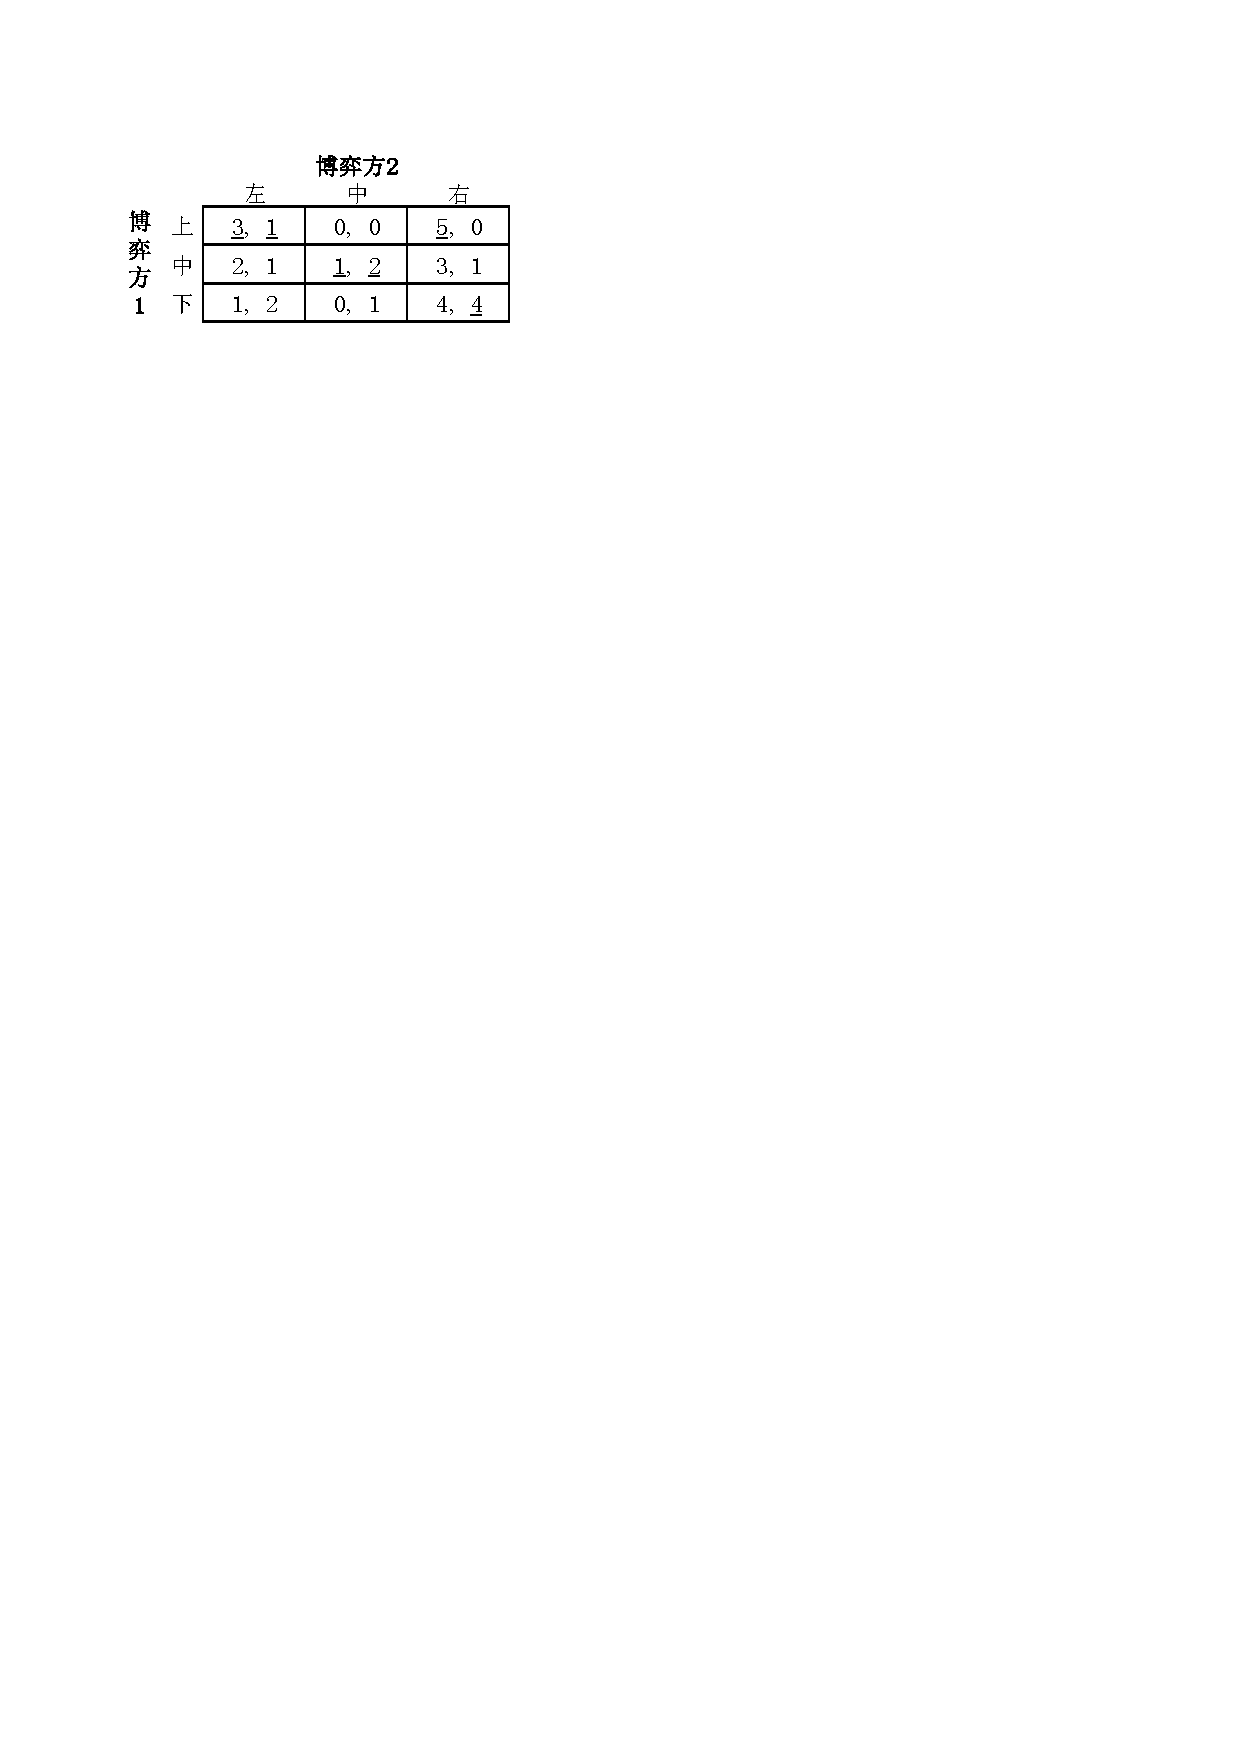
\includegraphics[scale=1]{Economic4.7.pdf}
    \caption{第7题}
\end{figure}
\begin{solution}
    (1). 根据划线法可以得出两个纯策略纳什均衡(上, 左)和(中, 中), Pareto上策均衡为(下, 右).
    
    博弈方1第一次选择下, 若结果为(下, 右), 则第二次选中; 否则, 由报复机制, 第二次选上.

    博弈方2第一次选择右, 若结果为(下, 右), 则第二次选左; 否则, 由报复机制, 第二次选中.

    (2). 若(下, 左)的得益改为$(1, 5)$, 对于博弈方2来说, (下, 左)是Pareto上策, 则选右的概率减小, 从而选(下, 右)的概率减小.

    (3). 条件为: (下, 右)是Pareto上策, 且双方都存在当决策结果不为(下, 右)时报复对方的策略.
\end{solution}
\paragraph{8.}求出下列得益矩阵表示的静态博弈的纳什均衡, 并说明有限次和无限次重复该博弈时两博弈方的均衡策略.
\begin{figure}[htbp]
    \centering
    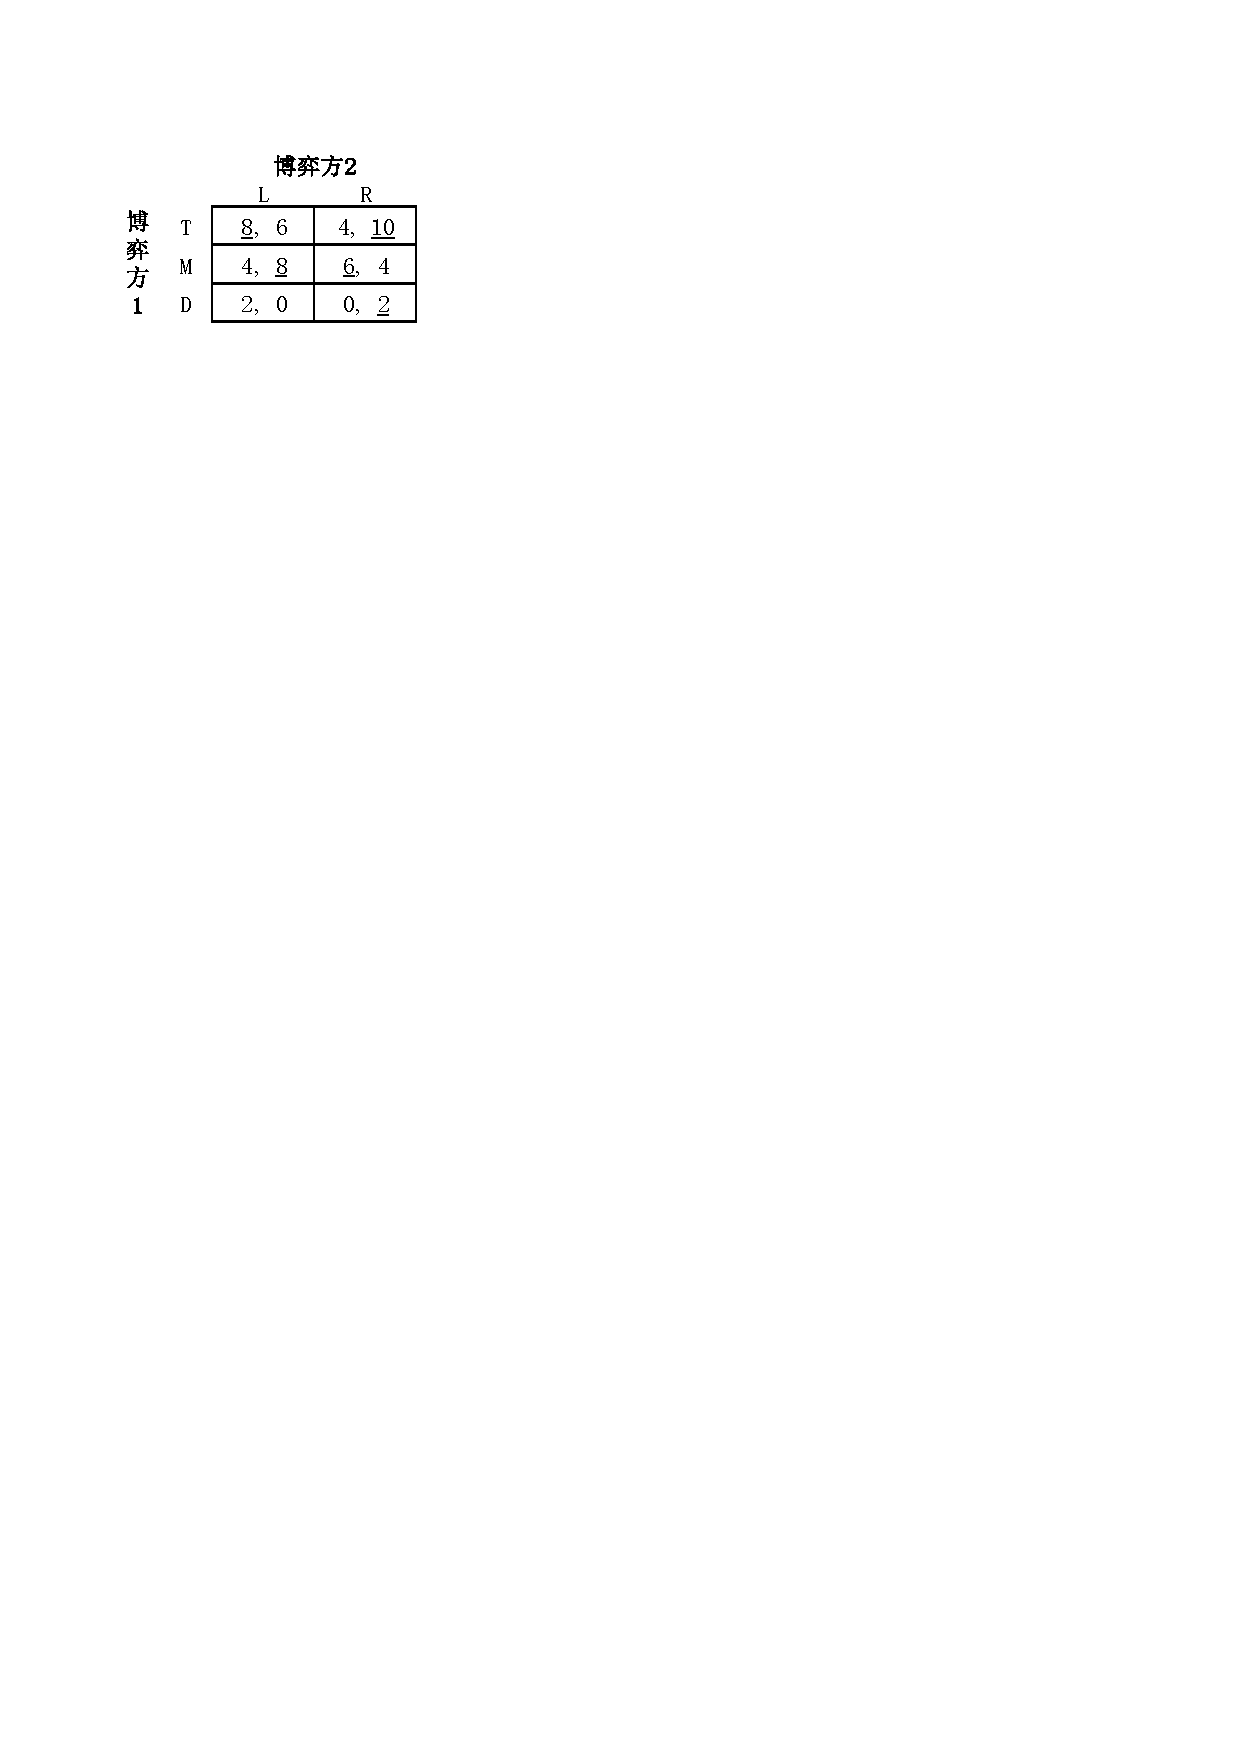
\includegraphics[scale=1]{Economic4.8.pdf}
    \caption{第8题}
\end{figure}
\begin{solution}
    根据划线法得知, 该博弈没有纯策略纳什均衡, 对于博弈方1来说, D策略是严格下策, 故将其删去. 设博弈方选$T, M$的概率分别为$P_T, P_M$, 博弈方2选$L, R$概率分别为$P_L, P_R$, 则
    \begin{equation*}
        \begin{cases}
            6P_T+8P_M = 10P_T+4P_M,\\
            P_T+P_M = 1,\\
            8P_L+4P_R=4P_L+6P_R,\\
            P_L+P_R = 1.
        \end{cases}
        \Rightarrow\quad\begin{cases}
            P_T = P_M = \frac{1}{2},\\
            P_L = \frac{1}{3},\add\\
            P_R = \frac{2}{3}.
        \end{cases}
    \end{equation*}
    由于上述博弈是没有纯策略纳什均衡的严格竞争博弈, 所以在有限次和无限次重复该博弈时, 两博弈方的均衡侧率都是简单重复原博弈的混合策略纳什均衡.
\end{solution}



% 下面给一些功能的写法
\iffalse
% 图片模板
\centerline{
    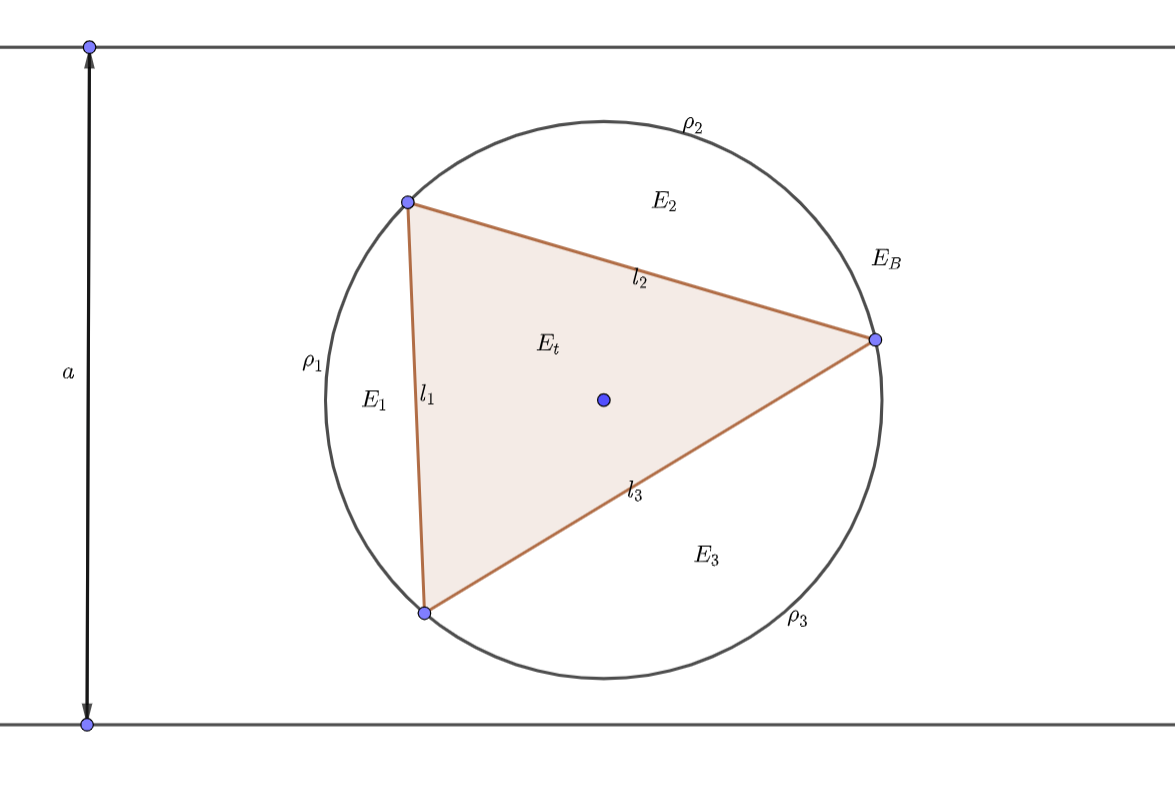
\includegraphics[width=0.8\textwidth]{figure.png}
}
% 表格模板
\renewcommand\arraystretch{0.8} % 设置表格高度为原来的0.8倍
\begin{table}[!htbp] % table标准
    \centering % 表格居中
    \begin{tabular}{p{1cm}<{\centering}p{1cm}<{\centering}p{3cm}<{\centering}p{5cm}<{\centering}} % 设置表格宽度
    %\begin{tabular}{cccc}
        \toprule
        $x_i$ & $f[x_1]$ & $f[x_i,x_{i+1}]$ & $f[x_i,x_{i+1},x_{i+2}]$ \\
        \midrule
        $x_0$ & $f(x_0)$ &                  &                          \\
        $x_0$ & $f(x_0)$ & $f'(x_0)$        &                          \\
        $x_0$ & $f(x_1)$ & $\frac{f(x_1)-f(x_0)}{x_1-x_0}$ & $\frac{f(x_1)-f(x_0)}{(x_1-x_0)^2}-\frac{f'(x_0)}{x_1-x_0}$\\
        \bottomrule
    \end{tabular}
\end{table}

\def\Log{\text{Log}} % 一个简单的宏定义
$\Log$ % 调用方法
\fi

\end{document}